\documentclass[a4j]{jarticle}
\usepackage[dvipdfmx]{graphicx}

\begin{document}

\title{$B7W;;5!2J3X<B835Z$S1i=,(B1 $BJs9p=q(B\\ 
% $B"-$3$3$K2]BjHV9f$r5-F~(B
\bf $B2]Bj(B11}
% $B"-$3$3$K<+J,$N;aL>$r5-F~(B
\author{$B?yK\IwEM(B \\
$B3X@RHV9f(B: 1029232337}
\$B@>Nq(B
% $B"-$3$3$KDs=PF|$r5-F~(B
\date{$BDs=PF|(B: \today}
%\date{$BDs=PF|(B: 1998$BG/(B6$B7n(B30$BF|(B}
\maketitle

\section{$B30It;EMM(B}
\begin{verbatim}
$ ./gya-tasukete11
\end{verbatim}
$BI8=`F~NO$+$iF~NO$r<u$1<h$k(B. 1$B9TL\$K%=!<%F%#%s%0%b%8%e!<%k$NHV9f$r(B, 2$B9TL\0J9_$K%=!<%H$9$k%G!<%?$r6uGr$^$?$O2~9T6h@Z$j$rM?$($k(B.\\
$B;XDj$7$?%=!<%F%#%s%0%b%8%e!<%k$rMQ$$$FF~NO$5$l$?%G!<%?$r%=!<%H$7(B, $B%=!<%H$7$?%G!<%?$rI8=`=PNO$K=PNO$9$k(B.\\
\\
$B%=!<%F%#%s%0%b%8%e!<%k$NHV9f$O(B, $B$=$l$>$l(B 0 $B$O%P%V%k%=!<%H%b%8%e!<%k(B, 1 $B$O%/%$%C%/%=!<%H%b%8%e!<%k$KBP1~$9$k(B.\\
\\
$B%=!<%F%#%s%0%b%8%e!<%k$NHV9f$O0J2<$N$h$&$K%3%^%s%I0z?t$N(B1$BHVL\$KM?$($k$3$H$b$G$-$k(B.\\

\begin{verbatim}
$ ./gya-tasukete11 0 < data
\end{verbatim}

\subsection{$B%W%m%0%i%`L>!J%3%^%s%IL>!K(B}
gya-tasukete11

\subsection{$B%W%m%0%i%`0z?t(B}
$B%=!<%F%#%s%0%b%8%e!<%k$NHV9f(B ($BM?$($J$$>l9g$O(B, $BI8=`F~NO$+$i<u$1<h$k(B).\\

\subsection{$B%W%m%0%i%`$N5!G=(B}

1$B9TL\$OMQ$$$k%=!<%F%#%s%0%b%8%e!<%k$NHV9f(B, 2$B9TL\0J9_$KF~NO%G!<%?$rI8=`F~NO$+$i<u$1<h$k(B.\\
$B%=!<%F%#%s%0%b%8%e!<%k$K$O%P%V%k%=!<%H(B, $B%/%$%C%/%=!<%H$rMQ$$$k$3$H$,$G$-$k(B.\\
$BF~NO%G!<%?$r;XDj$5$l$?%=!<%F%#%s%0%b%8%e!<%k$G%=!<%H$7(B, 1$B9T$K(B10$B%3$:$D=PNO$9$k(B.\\

% $B?t9TDxEY$G@bL@!%;29M;qNA$N(B dead copy $B$H$J$i$J$$$h$&!$G[N8$;$h!%(B

\subsection{$BF~=PNO%G!<%?$*$h$S;2>H%U%!%$%k(B}

$B;XDj$5$l$?F~NO%G!<%?$rMQ$$$?(B.\\

\subsection{$B<B9TNc(B}
$B%P%V%k%=!<%H%b%8%e!<%k$r;XDj$7F~NO%G!<%?$rM?$($kNc$r<($9(B.\\

\subsubsection{$BF~NO(B}
\begin{verbatim}
0
3198 4399 2962 1572 2704 395 2537 46 672 0
12137 0 300 568 1794 498 3015 1284 1299 1439
($BN,(B)
712 1964 828 894 2293 2560 505 1202 432 0
0 2 0 0 1035 946 2616 2426 1147 1371
\end{verbatim}
\subsubsection{$B=PNO(B}
\begin{verbatim}
       0       0       0       0       0       0       0       0       0       0
       0       0       0       0       0       0       0       0       0       0
($BN,(B)
\end{verbatim}
% $BE57?E*$J<B9TNc$r<($9!%(B

\subsection{$B%(%i!<>r7o$H%(%i!<=hM}5!G=(B}
$BIT@5$J%=!<%F%#%s%0%b%8%e!<%kHV9f$,F~NO$KM?$($i$l$?$H$-I8=`%(%i!<$K%(%i!<%a%C%;!<%8$r=PNO$9$k(B.\\
\subsubsection{$BF~NONc(B}
\begin{verbatim}
$ ./gya-tasukete11 -1
\end{verbatim}

\subsubsection{$B%(%i!<=PNO(B}
\begin{verbatim}
$B$=$N%=!<%F%#%s%0%b%8%e!<%kHV9f$OIT@5$G$9(B: -1
\end{verbatim}
% $BJ#?t$N%(%i!<>r7o$,$"$k>l9g$O(B {enumerate} $B$^$?$O(B {itemize} $B$G5-=R!%(B
% $B%(%i!<=hM}$NNc$b<($9!%(B

\subsection{$B%"%k%4%j%:%`$NN.$l?^(B}
\begin{center}
  \includegraphics[width=100mm]{main.pdf}
\end{center}

\subsubsection{$B%P%V%k%=!<%H(B}
\begin{center}
  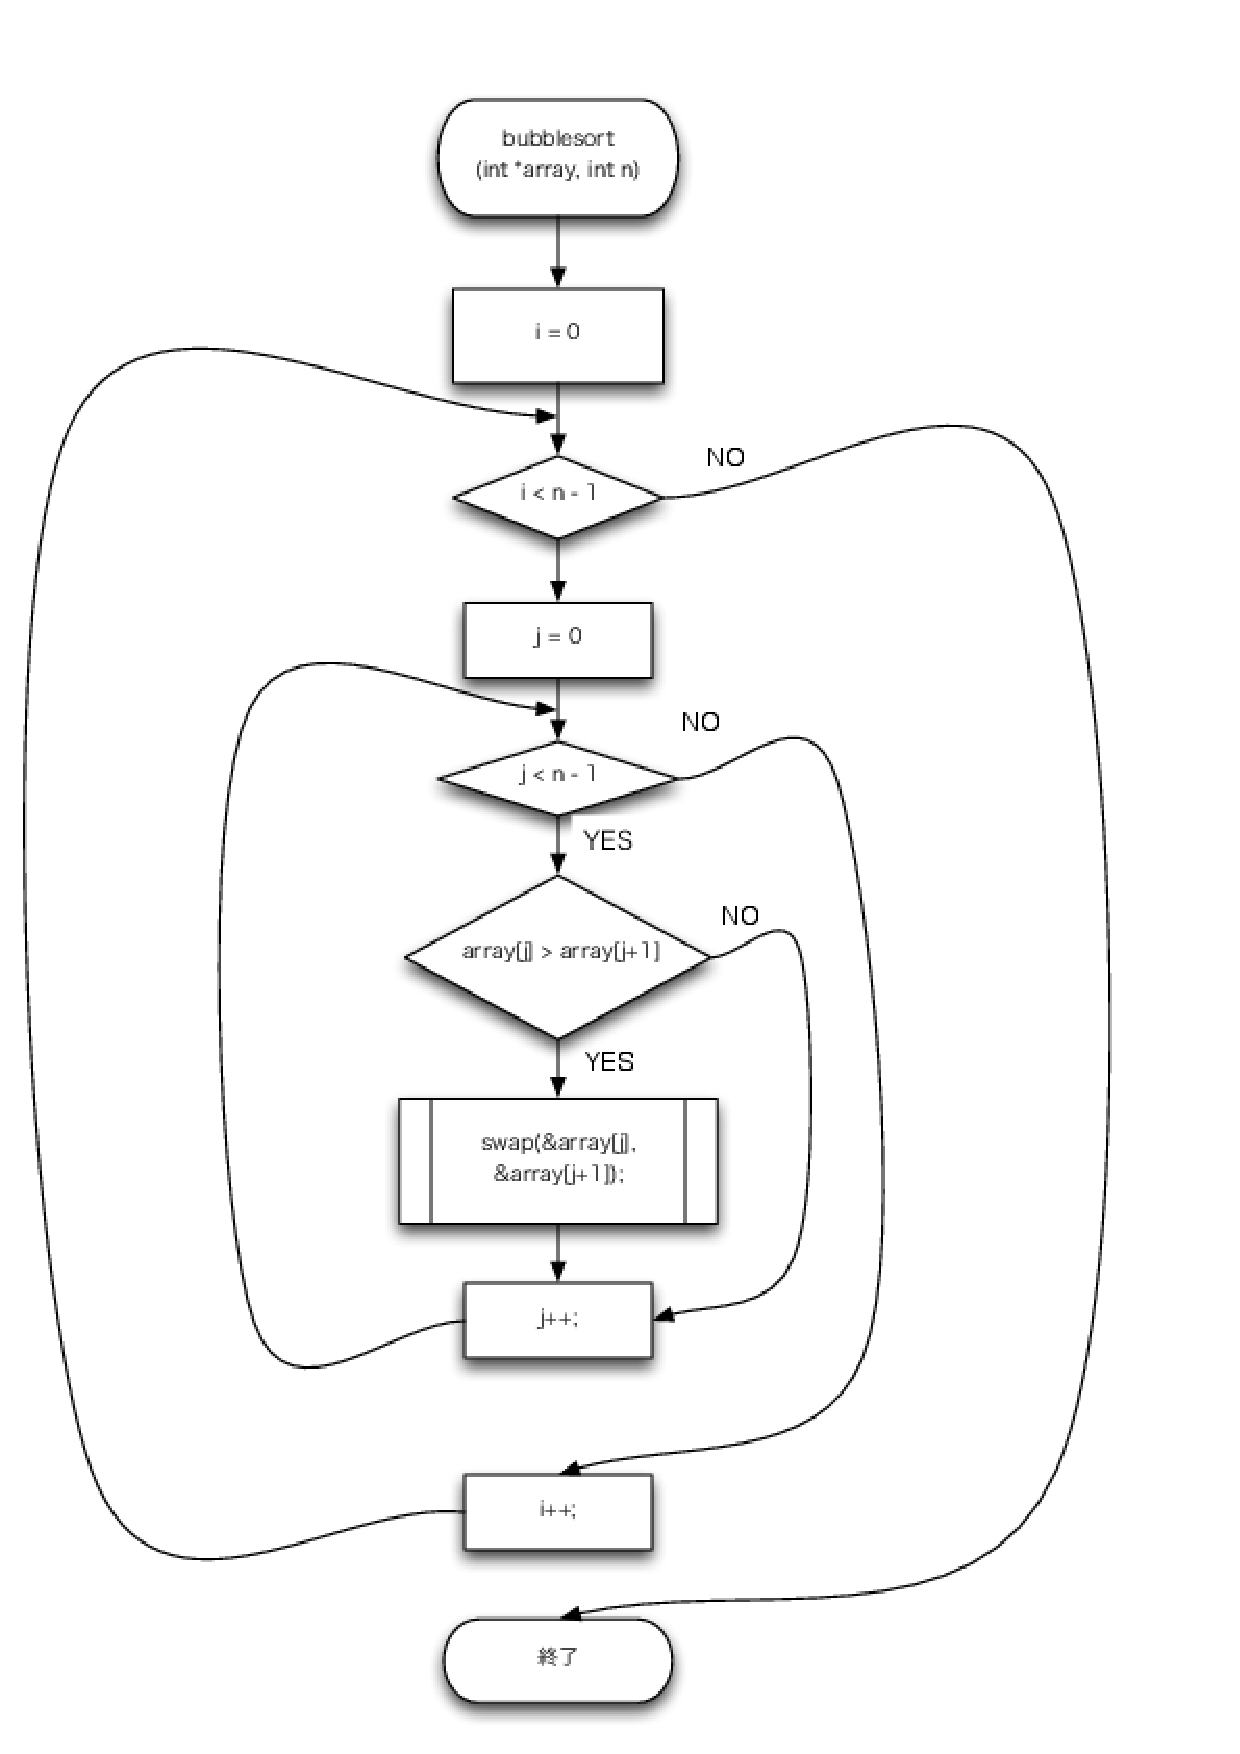
\includegraphics[width=100mm]{bubblesort.pdf}
\end{center}

\subsubsection{$B%/%$%C%/%=!<%H(B}
\begin{center}
  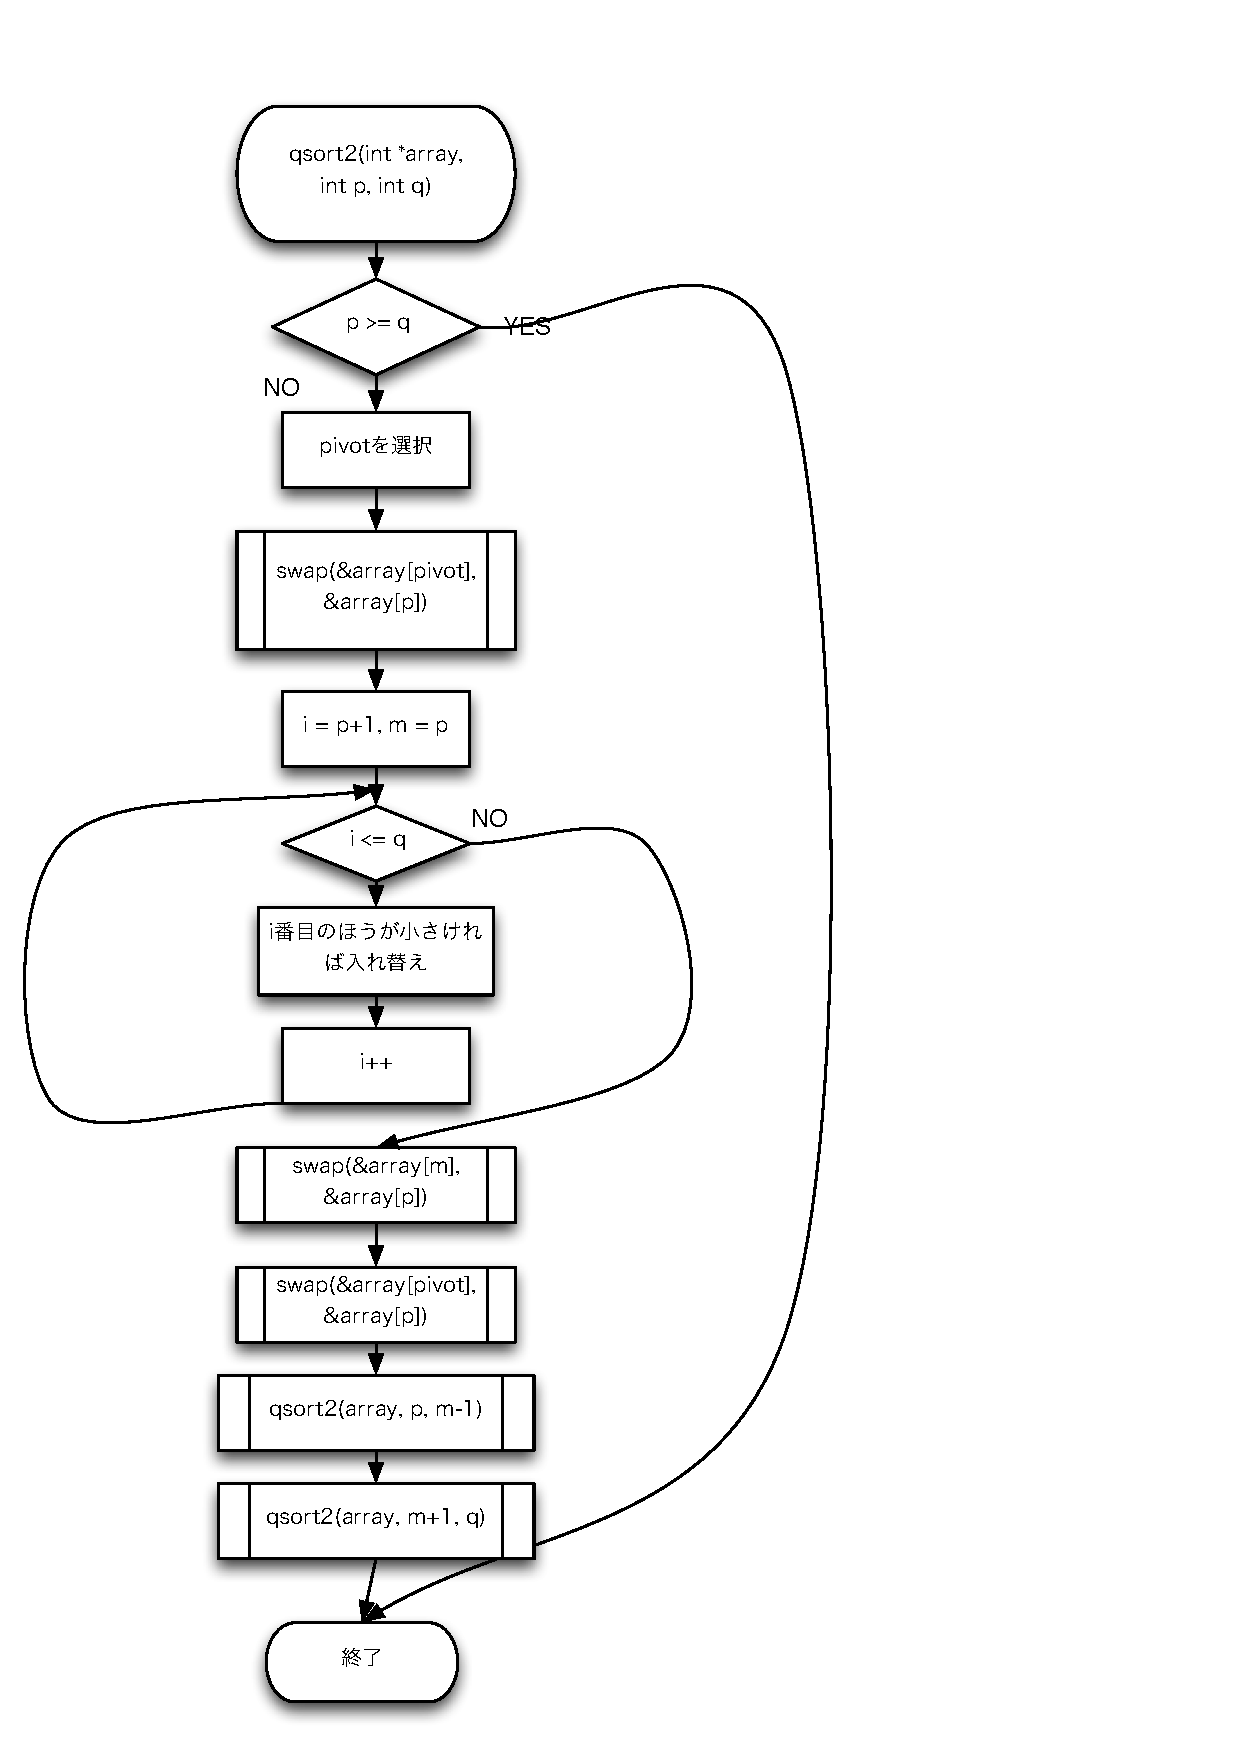
\includegraphics[width=100mm]{qsort.pdf}
\end{center}

\section{$BFbIt;EMM(B}
% $BFbIt;EMM$H$O!$30It;EMM$K<($5$l$?5!G=!$?6Iq$$$r%W%m%0%i%`$,$$$+$K<B8=(B
% $B$7$F$$$k$+!$%W%m%0%i%`$N9=@.$dO@M}$r5-=R$7$?$b$N$G$"$k!%(B

\subsection{$B%b%8%e!<%k;EMM(B}

\subsubsection{swap}
\begin{verbatim}
void swap(int *a, int *b);
\end{verbatim}

\begin{description}
\item[$B%b%8%e!<%k$N5!G=(B]
$B;XDj$5$l$?(B2$B$D$NG[Ns%]%$%s%?$NCf?H$rF~$lBX$($k(B.\\

\item[$B%b%8%e!<%k%$%s%?%U%'!<%9(B]\mbox{}\\[-7mm]
\begin{enumerate}
\item[$B0z?t(B] int$B7?G[Ns%]%$%s%?(Ba,b
\item[$B=PNO(B] void
\end{enumerate}
% $B3F0z?t$NL>A0!$7?!$MQES$N@bL@!$F~=PNO$NJL!(JV$jCM$N7?!$MQES$N@bL@$r(B
% {enumerate} $B$G5-=R!%(B

\item[$BFbItJQ?t(B]\mbox{}\\[-7mm]
\begin{enumerate}
\item int temp$B$O0l;~JQ?t(B.
\end{enumerate}
% $B3FJQ?t$NL>A0!$7?!$MQES$N@bL@$r(B {enumerate} $B$G5-=R!%(B
% $B9=B$BN$K$D$$$F$O$=$N%U%#!<%k%I$K$D$$$F$bF1MM$K5-=R$9$k!%(B

\item[$BO@M}(B]\mbox{}\\[-7mm]
\begin{verbatim}
$B0l;~JQ?t$r@k8@(B;
$B0l;~JQ?t$rMQ$$$F(Ba$B$H(Bb$B$rF~$lBX$($k(B;
\end{verbatim}
\end{description}


\subsubsection{bubblesort}
\begin{verbatim}
void bubblesort(int *array, int n);
\end{verbatim}
\begin{description}
\item[$B%b%8%e!<%k$N5!G=(B]
$BM?$($i$l$?%5%$%:(Bn$B$NG[Ns$r%P%V%k%=!<%H$9$k(B. 

\item[$B%b%8%e!<%k%$%s%?%U%'!<%9(B]\mbox{}\\[-7mm]
\begin{enumerate}
\item[$B0z?t(B] array: int$B7?G[Ns%]%$%s%?(B
\item[$B=PNO(B] void
\end{enumerate}

\item[$BO@M}(B]\mbox{}\\[-7mm]
\begin{verbatim}
for (0 <= i < n - 1)
  for (0 <= j < n - 1)
    if j+1$BHVL\$h$j$b(Bj$BHVL\$N$[$&$,Bg$-$$(B
      swap(j$BHVL\(B, j+1$BHVL\(B);
\end{verbatim}
% C $B9=J8$rMQ$$$?5?;w%3!<%I$K$h$k<jB3$-$N5-=R!%(B
% \begin{verbatim} ... \end{verbatim} $B$G0O$`$H$h$$!%(B
\end{description}


\subsubsection{qsort2}
\begin{verbatim}
void qsort2(int *array, int p, int q);
\end{verbatim}
\begin{description}
\item[$B%b%8%e!<%k$N5!G=(B]
$BG[Ns(Barray$B$r(Bp$B$+$i(Bq$B$^$G$NHO0O$G%/%$%C%/%=!<%H$9$k(B.

\item[$B%b%8%e!<%k%$%s%?%U%'!<%9(B]\mbox{}\\[-7mm]
\begin{enumerate}
\item[$B0z?t(B] array: int$B7?G[Ns%]%$%s%?(B p,q: int$B7?6h4V(B
\item[$B=PNO(B] void
\end{enumerate}

\item[$BFbItJQ?t(B]\mbox{}\\[-7mm]
\begin{enumerate}
\item int pivot: $B%T%\%C%H(B
\end{enumerate}
% $B3FJQ?t$NL>A0!$7?!$MQES$N@bL@$r(B {enumerate} $B$G5-=R!%(B
% $B9=B$BN$K$D$$$F$O$=$N%U%#!<%k%I$K$D$$$F$bF1MM$K5-=R$9$k!%(B

\item[$BO@M}(B]\mbox{}\\[-7mm]
\begin{verbatim}
if (p >= q)
  return;

$B%T%\%C%H$rG[Ns$+$iE,Ev$KA*$V(B;
$BG[Ns$NCf?H$r%T%\%C%H$NA0$K%T%\%C%H$h$j$b>.$5$$?t$r(B,$B8e$m$K%T%\%C%H$h$j$bBg$-$$?t$,$/$k$h$&$K$9$k(B;

qsort2(p$B$+$i%T%\%C%H$ND>A0(B);
qsort2($B%T%\%C%H$N8e$m$+$i(Bq$B$^$G(B);
\end{verbatim}
% C $B9=J8$rMQ$$$?5?;w%3!<%I$K$h$k<jB3$-$N5-=R!%(B
% \begin{verbatim} ... \end{verbatim} $B$G0O$`$H$h$$!%(B
\end{description}


\subsubsection{w\_qsort2}
\begin{verbatim}
void w_qsort2(int *array, int n);
\end{verbatim}
\begin{description}
\item[$B%b%8%e!<%k$N5!G=(B]\mbox{}\\
$BM?$($i$l$?%5%$%:(Bn$B$NG[Ns$r%/%$%C%/%=!<%H$9$k(B.\\$BFbIt$G$d$C$F$k$3$H$O(Bqsort2$B$K0z?t$rEO$9$@$1(B.\\
\end{description}


\subsubsection{input}
\begin{verbatim}
void input(int *array, int *n);
\end{verbatim}

\begin{description}
\item[$B%b%8%e!<%k$N5!G=(B]
$BI8=`F~NO$+$i%G!<%?$r<u$1<h$k(B.\\

\item[$B%b%8%e!<%k%$%s%?%U%'!<%9(B]\mbox{}\\[-7mm]
\begin{enumerate}
\item array$B$OF~NO%G!<%?Ns(B
\item n$B$O(Bint$B7?%]%$%s%?(B. $BF~NO%G!<%?$N%5%$%:$rBeF~$9$k(B.
\end{enumerate}

\item[$BO@M}(B]\mbox{}\\[-7mm]
\begin{verbatim}
int i = 0;
while ($B0l9TFI$_<h$k(B) {
  while ($B?t$r$R$H$DFI$_<h$C$F(Barray$B$KBeF~(B)
    i++;
}

*n = i;
\end{verbatim} 
\end{description}


\subsubsection{output}
\begin{verbatim}
void output(int *array, int n);
\end{verbatim}
\begin{description}
\item[$B%b%8%e!<%k$N5!G=(B]
$BI8=`=PNO$K(Barray$B$NCf?H$r@07A$7$F=PNO$9$k(B.\\

\item[$B%b%8%e!<%k%$%s%?%U%'!<%9(B]\mbox{}\\[-7mm]
\begin{enumerate}
\item array$B$OF~NO%G!<%?Ns(B
\item n$B$OF~NO%G!<%?$N%5%$%:(B
\end{enumerate}

\item[$BO@M}(B]\mbox{}\\[-7mm]
\begin{verbatim}
for ($BG[Ns(Barray)
  $BCf?H$r=PNO(B;
\end{verbatim}
\end{description}

\section{$BBg0hJQ?t(B}
$B$J$7(B
\section{$B%W%m%0%i%`$NI>2A(B}
$B%=!<%F%#%s%0%b%8%e!<%kKh$K7WB,$7$?<B9T;~4V$r:\$;$k(B.\\
\begin{tabular}[t]{|c|c|}
\hline
$B%"%k%4%j%:%`(B&$B;~4V(B(s)\\
\hline
$B%P%V%k%=!<%H(B&0.85\\
\hline
$B%/%$%C%/%=!<%H(B&0.01\\
\hline
\end{tabular}


\section{$B%W%m%0%i%`3+H/$N7P2a(B}
\begin{description}
\item[$BLdBj$NJ,@O$H2rK!$N8!F$(B] 10$BJ,(B
\item[$B%b%8%e!<%k9=B$@_7W(B] 10$BJ,(B
\item[$B%b%8%e!<%kFbO@M}@_7W(B/$B%W%m%0%i%_%s%0(B] 10$BJ,(B
\item[$B%W%m%0%i%`%F%9%H!$%G%P%C%0(B] 10$BJ,(B
\item[$B;EMM=q$N:n@.(B] 1$B%v7n(B
\end{description}
% $B%W%m%0%i%`3+H/$N3FCJ3,$GMW$7$?;~4VG[J,!J9)?t!K$N35N,$r5-$9!%(B
% $B$"$H$b$I$j$,$"$C$?>l9g$O$=$N>u67$K$D$$$F$b@bL@$9$k!%(B
% $B3FCJ3,$H$O<!$NDL$j!'(B
% 1. $BLdBj$NJ,@O$H2rK!$N8!F$(B
% 2. $B%b%8%e!<%k9=B$@_7W(B
% 3. $B%b%8%e!<%kFbO@M}@_7W(B/$B%W%m%0%i%_%s%0(B
% 4. $B%W%m%0%i%`%F%9%H!$%G%P%C%0(B
% 5. $B;EMM=q$N:n@.(B

\section{$B46A[(B}
$B;EMM=q=q$/$N$O%/%=(B.\\

\newpage
\section*{$BIUO?(B}
\begin{verbatim}
#include <stdio.h>
#include <stdlib.h>
#define MAX_N 100000
#define MAX_OUTPUT 10
#define FUNC_N 2

void swap(int *a, int *b);
void bubblesort(int *array, int n);
void qsort2(int *array, int p, int q);
void w_qsort2(int *array, int n);
void input(int *array, int *n);
void output(int *array, int n);


int main(int argc, char *argv[]) {
  char buf[1000];
  int array[MAX_N];
  int n, func_i;

  void (*func[FUNC_N])(int *, int) = { bubblesort, w_qsort2 };

  // batch mode
  if (argc >= 2) {
    sscanf(argv[1], "%d", &func_i);
  } else {
    fgets(buf, 1000, stdin);
    sscanf(buf, "%d", &func_i);
  }

  if (!(0 <= func_i && func_i < FUNC_N)) {
    fprintf(stderr, "$B$=$N%=!<%F%#%s%0%b%8%e!<%kHV9f$OIT@5$G$9(B: %d\n", func_i);
    exit(1);
  }

  input(array, &n);
  func[func_i](array, n);
  output(array, n);

  return 0;
}

// $BF~NO9T?t$rJV$9(B
void input(int *array, int *n) {
  char buf[MAX_N];
  int i = 0, start_i, read_i;

  while(fgets(buf, MAX_N, stdin) != NULL) {
    start_i = read_i = 0;
    while (sscanf(buf + start_i, "%d %n", &array[i++], &read_i) != EOF) {
      start_i += read_i;
    }
  }

  *n = i;
}

void output(int *array, int n) {
  int i;
  for(i = 0; i < n; i++) {
    if ((i+1) % MAX_OUTPUT == 0) {
      printf("%8d\n", array[i]);
    } else {
      printf("%8d", array[i]);
    }
  }
  printf("\n");
}

// array$B$r6h4V(Bp,q$B$G%=!<%H$9$k(B
// p <= q
void qsort2(int *array, int p, int q) {
  int i, m, pivot = p;

  if (p >= q) 
    return;

  // $B@hF,$+$i(B3$B$D$H$C$F$=$NCf1{CM$r%T%\%C%H$K$9$k(B
  if (p - q >= 2) {
    for (i = 0; i < 3; i++) {
      if ((array[p+(i-1)%3] < array[i] && array[i] < array[p+(i+1)%3]) || (array[p+(i+1)%3] < array[i] && array[i] < array[p+(i-1)%3])) {
        pivot = p;
      }
    }
  }

  swap(&array[pivot], &array[p]);

  for (i = p+1, m = p; i <= q; i++) {
    if (array[i] < array[p]) {
      swap(&array[++m], &array[i]);
    }
  }

  swap(&array[m], &array[p]);

  swap(&array[pivot], &array[p]);

  qsort2(array, p, m-1);
  qsort2(array, m+1, q);
}

void w_qsort2(int *array, int n) {
  qsort2(array, 0, n - 1);
}

void swap(int *a, int *b) {
  int temp = *a;
  *a = *b;
  *b = temp;
}

void bubblesort(int array[], int n) {
  int i, j;

  for (i = 0; i < n - 1; i++)
    for (j = 0; j < n - 1; j++) 
      if (array[j] > array[j+1])
        swap(&array[j], &array[j+1]);

}



\end{verbatim}

\end{document}
